
\section{\ref{rq:application-outside-testar}How can we set up the change detection as an application written outside of \testar?} \label{sec:components-explained}
The new application is written outside the \testar application. Doing so makes it possible to work without the context and dependencies of \testar and allows the application to be written in a language more known by the developer. The only dependency it has with \testar is the OrientDB graph database.

Besides OrientDB, the solution is divided into two major parts. A \testar proxy, named .NET server, and a new \testar analysis website. As the name suggests, they are built and created in Framework from Microsoft: .NET Core (version 6) \footnote{\url{https://dot.net}}. .NET is an open-source, cross-platform framework. An application created with .NET will run on Windows, Linux and macOS. 

\begingroup
\captionsetup{type=figure}
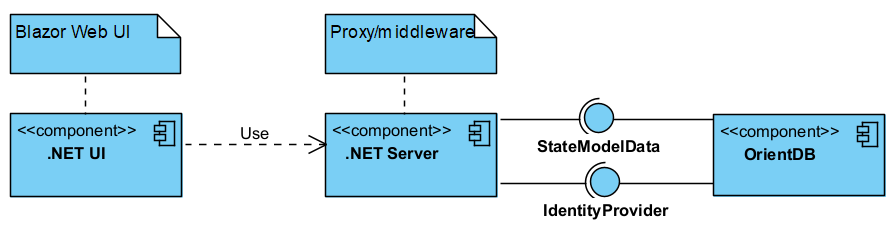
\includegraphics[scale=0.7]{images/server-ui-comp.png}
\captionof{figure}{.NET UI - Server and OrientDb component model (UML 2.0)}\label{fig:components}
\endgroup

Figure \ref{fig:components} shows the three components making up the system. The state model data that \testar generated is saved into the OrientDB graph database, and the .NET server uses the same database. The new \testar analysis website connects to the .NET server. In the following sections, the different components are explained. 

Since both the .NET server and the website are running .NET, they use the same core library. Using the same core library makes it easy to share code. As an extra benefit, the core library can be reused in other applications dedicated to a single task. 

\subsection{OrientDB Component}
OrientDB is the data storage for \testar. The new application presents the data to the user. In order to query the data, the \verb|REST| API of OrientDB is used. A \verb|POST| is sent to OrientDB with the query and parameters in the request's body. An example of the body is displayed in listing \ref{code:example-body}.

\begin{lstlisting}[language=xml, caption=Get AbstractStateModel by the model identifier, label=code:example-body]
{
  "command": "SELECT FROM AbstractStateModel WHERE modelIdentifier = :id",
  "parameters": {
    "id": "1chdi5230521708089"
  }
}
\end{lstlisting}

An alternative way of querying the data is using the query \verb|GET| operation. While it is easy to query the data, it is vulnerable to SQL injection since the parameters are directly used in the SQL query. Those parameters can be changed by user input. 

The current solution in which the queries are sent from the UI to the .NET server is not entirely foolproof either. For example, using the Burp Suite is still possible to alter the \verb|POST| message body and attack the OrientDB database. This issue can be circumvented by setting up \verb|REST| endpoints on the.NET Server that created the SQL calls on the server-side.

It is not recommended to expose the OrientDB database directly to a public network \cite{orientdb-security}. Besides the orientDb recommended best practices and issues accessing the database on a web frontend, a proxy/middleware component is built. The following section explains the .NET server in more detail. 

\subsection{.NET Server} \label{sec:net-server}
The .NET Server serves as a proxy between the new \testar analysis website and the existing OrientDB graph database. It also provides an easy to use endpoint for other to-be-build applications.

The need for the .NET Server was due to browser restrictions and limitations in accessing the database. Two issues arose when the UI was trying to connect to the database. The issue was \acrfull{cors}. CORS is a security feature in which a web server can permit or deny requests from a website if the request was not made from a trusted source \cite{cors}. By default OrientDB does not permit other websites to use their \verb|REST| endpoints \cite{orientdb-webserver}. It is possible to enable CORS in the OrientDB configuration, but before the .NET application can be used, administrators should edit the OrientDB configuration. Although it would solve the CORS issue, a second issue involving the cookie is not solved.

The second issue prevented the analysis website from accessing and reading the cookie created by OrientDB. OrientDB saves a cookie, the session token. Before a user can query the data, it needs to sign in to OrientDB. Sign in is accomplished by executing a \verb|GET| command to the \verb|/connect/database| endpoint and providing the username and password, encoded with the base64 algorithm, as an authentication header. The OrientDB will return a \verb|200 OK| response with a \verb|osessionid| in the response headers if the credentials are valid. The \verb|osessionid| authenticates the user on future calls.

It was impossible to retrieve the \verb|osessionid| header and reuse it in the further data retrieval calls. Because the web browser blocked the session header, we could store the users' credentials in local storage, making them available for retrieval with a Cross-Site Scripting attack. Section \ref{sec:auth} will look into authentication and authorisation in more detail.

The OrienDB URL and name of the \testar state model database are provided in the server configuration. Based on user feedback, it is also possible to enable muti-database features. Enabling the multi-database feature enables to user to specify the name of the database during logging in. For example, if the user wants to connect to the database \verb|TestarData| and the username is \verb|Kirk|, the username for sign in becomes: \verb|TestarData\Kirk|.

\subsection{New \testar analysis website}
With the \testar application, it is possible to open an analysis website \cite{thesisMulders}. This website provided several features like viewing the available state models, Test sequences and a graph engine created with Cytoscape.js. The user has to install \testar on their machine to view this analysis website. This thesis presents a new website that can be used outside the \testar application. It got a fresh look and feel, created with Bootstrap\footnote{\url{https://getbootstrap.com}} and a noticeable increase in performance. Figure \ref{fig:ui-home-page} show the renewed available models screen. 

\begingroup
\captionsetup{type=figure}
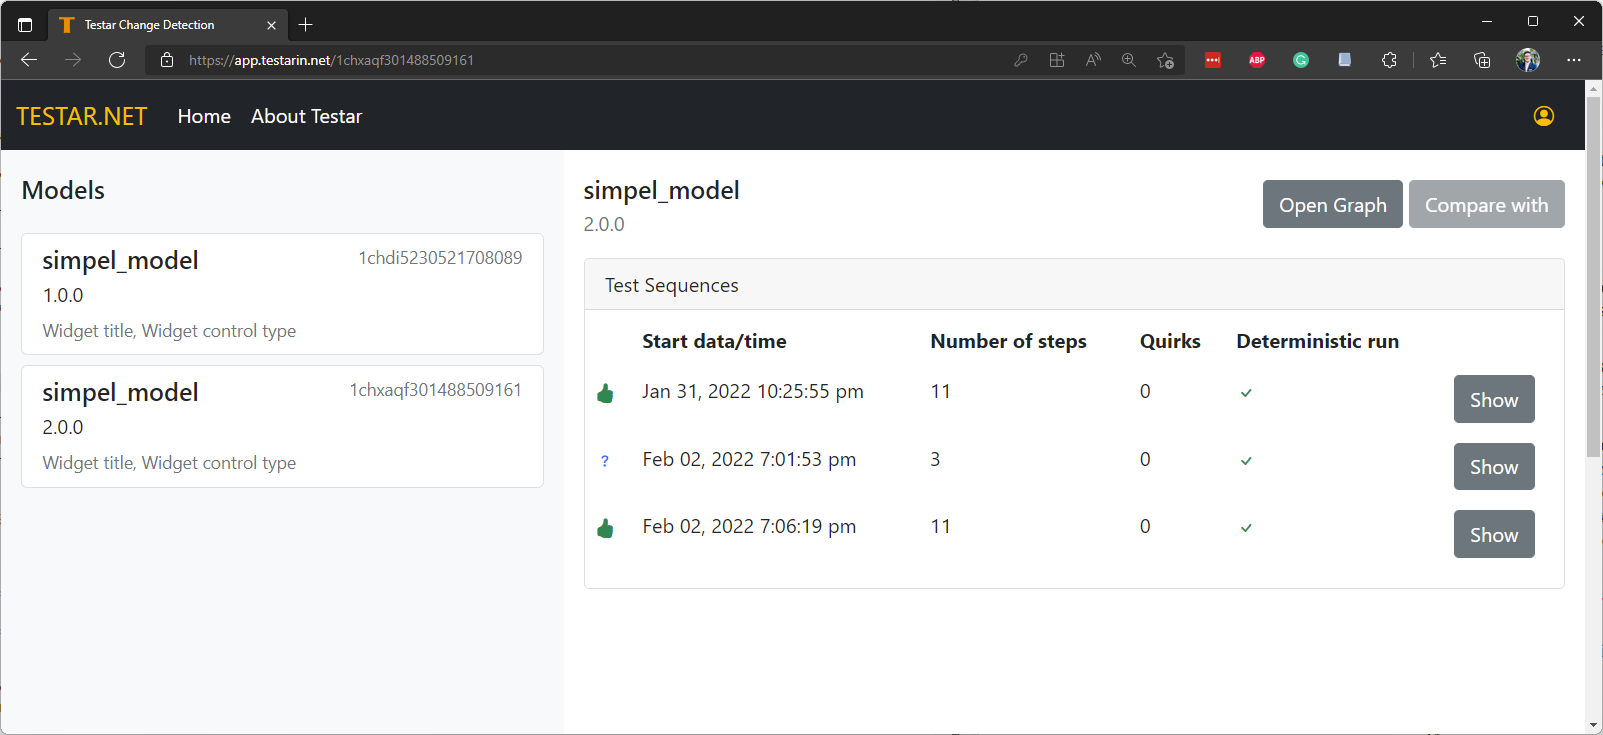
\includegraphics[scale=0.4]{images/ui-home-page.png}
\captionof{figure}{Available models in the new \testar website}\label{fig:ui-home-page}
\endgroup

The new \testar analysis website is created in Blazor. Blazor is an interactive web UI technology that allows running .NET code in the browser \cite{what-is-blazor}. For the graphical layer, Blazor uses HTML. Although some parts are still coded in Javascript, the application code is written in C\#. 

The code required to display the state graph, as shown in figure \ref{fig:graph-page}, has been copied from the original \testar source code. Besides the HTML layer and the retrieval of the raw model data, nothing has been altered. The graph engine is still using the Cytoscape.js library. 

\begingroup
\captionsetup{type=figure}
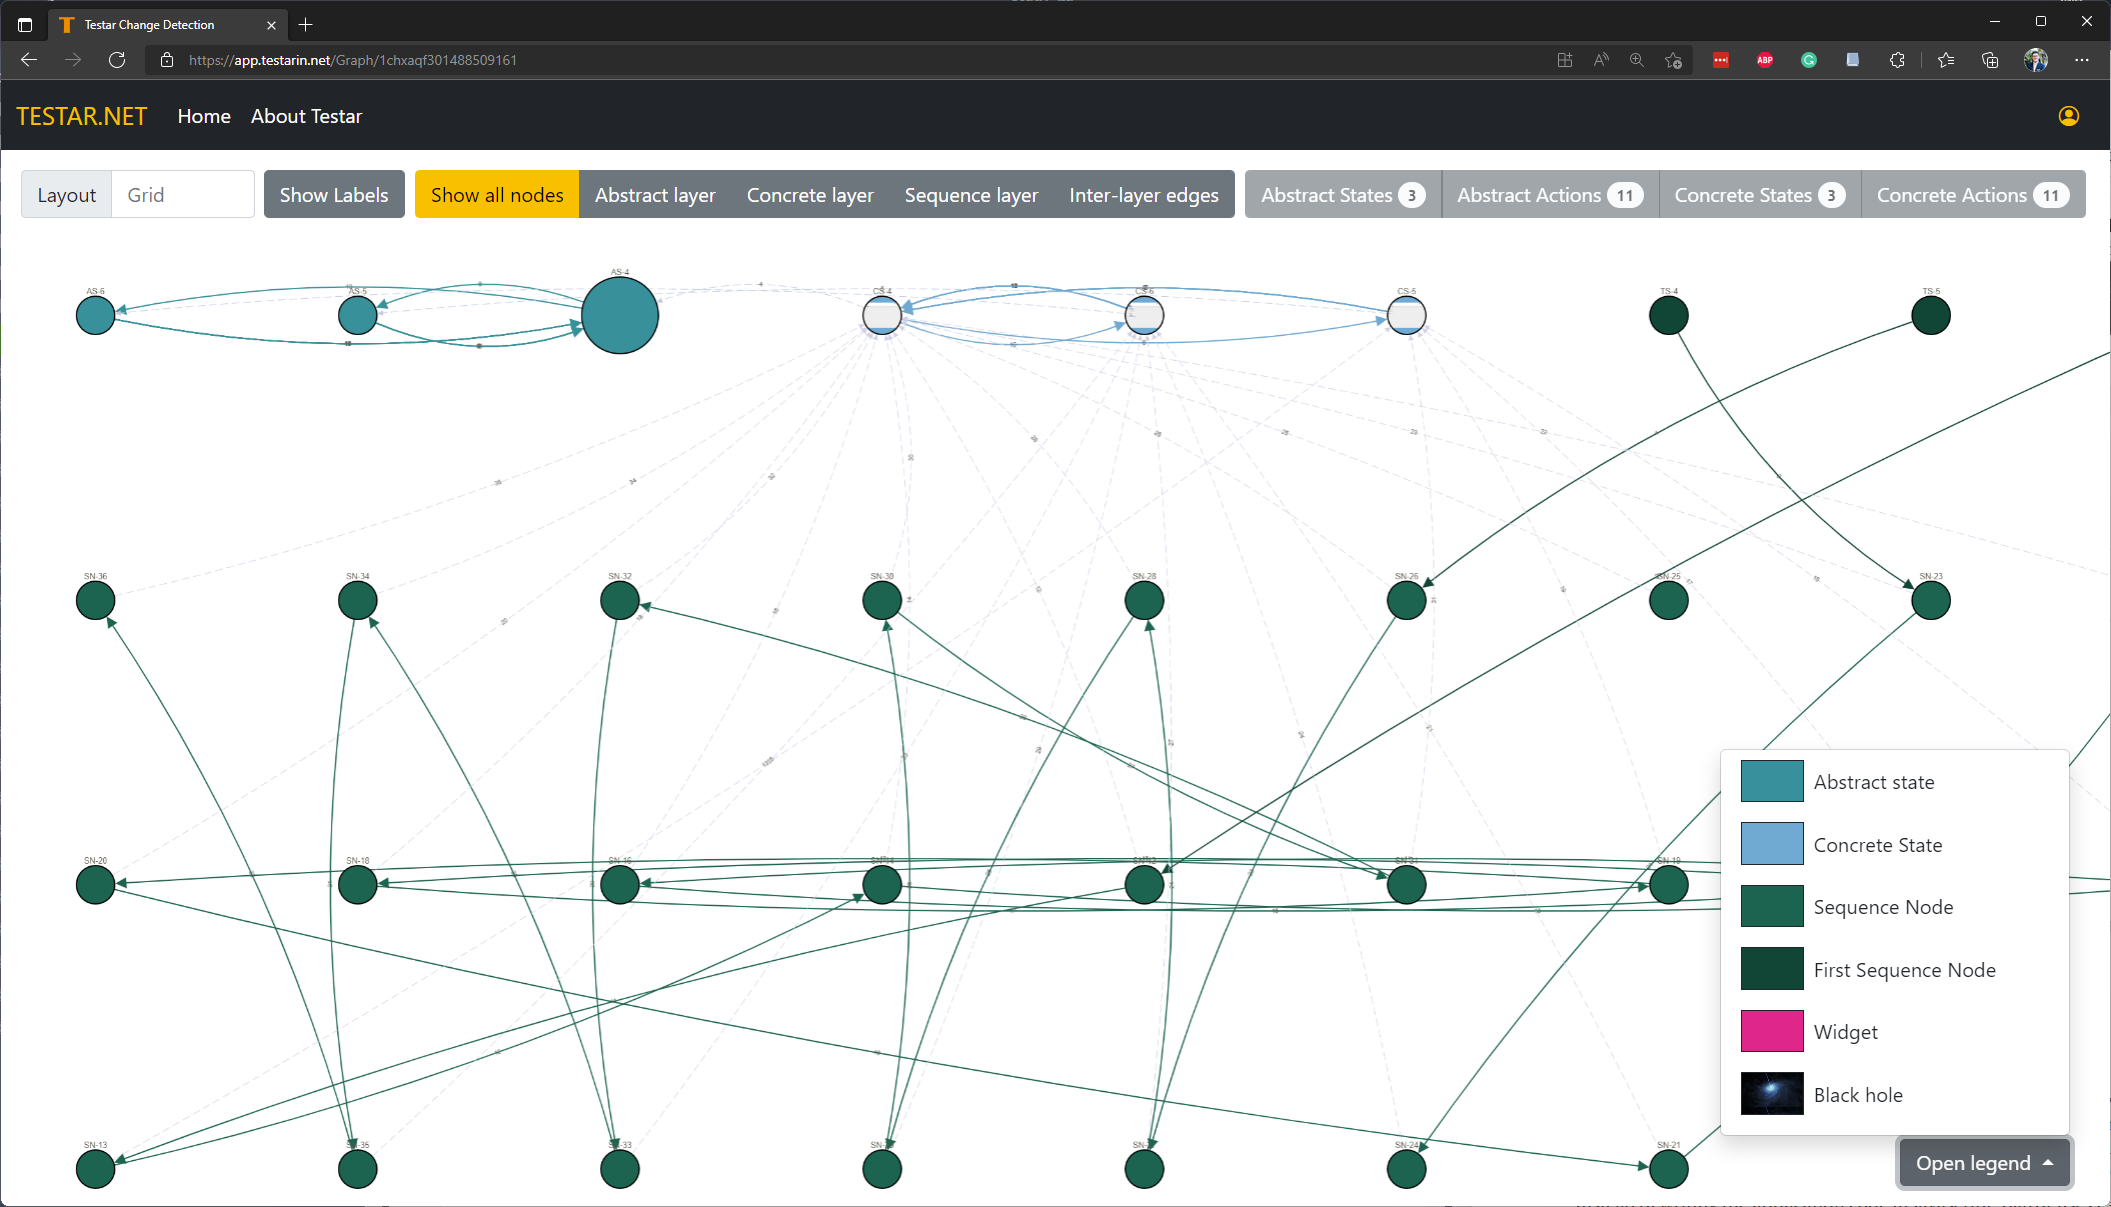
\includegraphics[scale=0.3]{images/graph-page.png}
\captionof{figure}{The new Graph page}\label{fig:graph-page}
\endgroup

\subsection{Authentication \& Authorisation} \label{sec:auth}
The .NET server helps with solving the security issues mentioned in ref{sec:net-server}  while still providing a secure and open authentication endpoint. External applications that want to use the endpoints must first authenticate with the .NET server upon it will return a \acrfull{jwt}. A JWT is a \textit{"compact, URL-safe means of representing claims to be transferred between two parties."} \cite{jones2015json}.

Before the user can use the \testar analysis website, it must authenticate itself. Figure \ref{fig:auth-sd} shows the sequence diagram of how the authentication flow is handled. Since the user identities are stored in the identity provider of the graph database, it is essential to note that the .NET server does neither handle authentication nor authorisation. The OrientDB Server handles the authentication and authorisation. The figure shows that the .NET server proxies the credentials and returns a JWT with the \verb|osessionid| as data. When the user provides incorrect credentials, the OrientDB will return a \verb|401 Unauthorised|, and the .NET server will return that status code.

\begingroup
\captionsetup{type=figure}
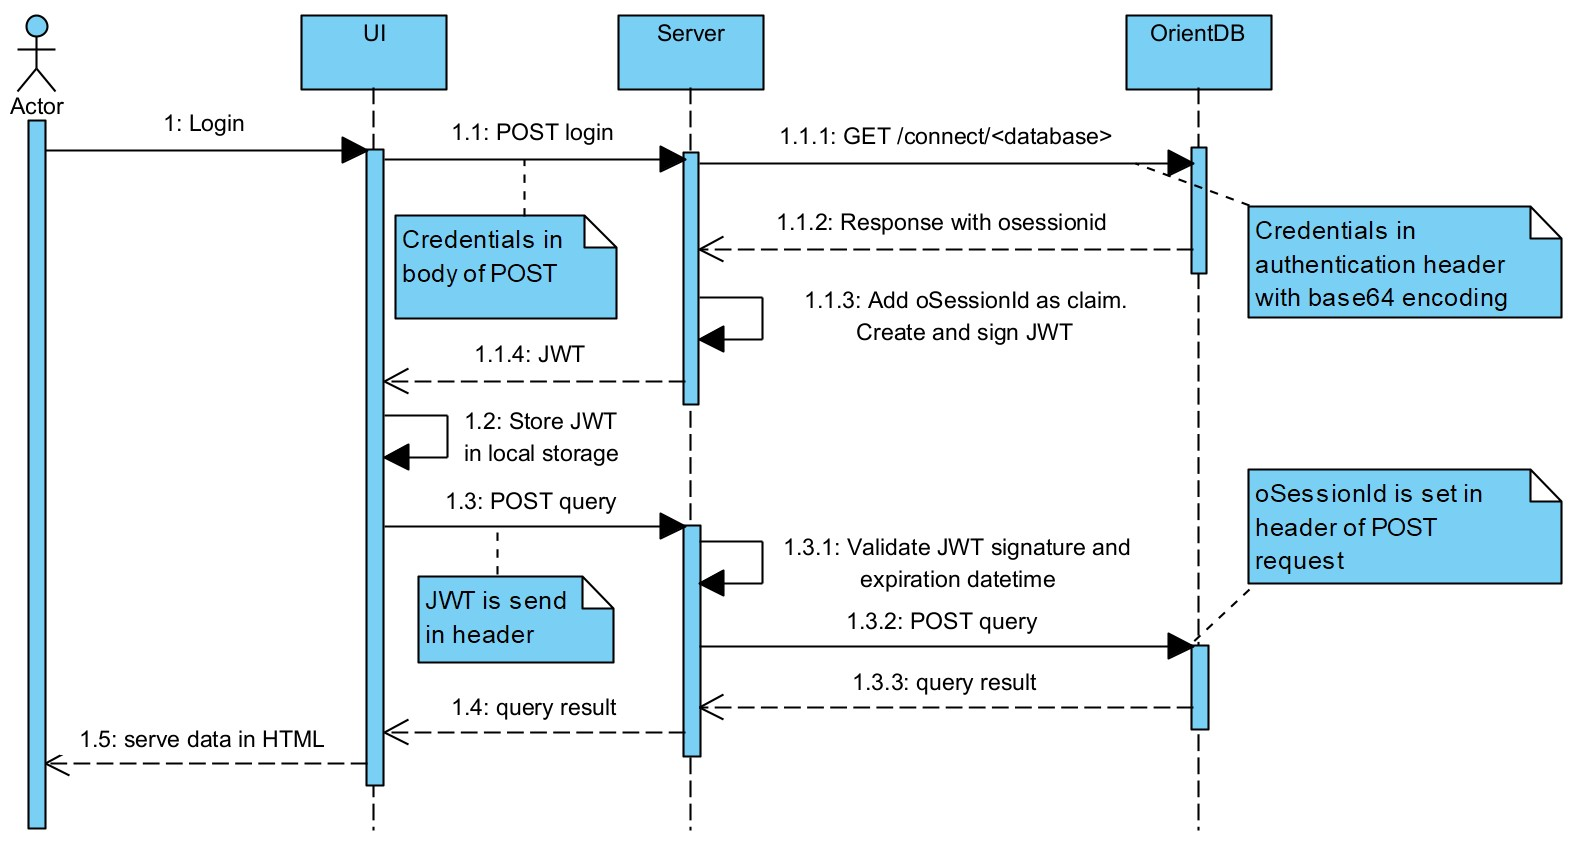
\includegraphics[scale=0.4]{images/authentication-sd.png}
\captionof{figure}{Authentication sequence (UML 2.0)}\label{fig:auth-sd}
\endgroup

An example of the JWT generated by the .NET server is displayed in listing \ref{code:jwt}. The JWT can be decoded by anyone, for example, with a website like \url{https://jwt.io}. The corresponding header and payload are displayed in listing \ref{code:jwt-payload}. In the JWT, two dots are visible, showing the three sections of the token. The first section is dedicated to the header information (lines 1-4 in listing \ref{code:jwt-payload}). The middle section contains the payload (lines 5-12 in listing \ref{code:jwt-payload}). The third and last section contains the signing information, validating the token. 

\begin{lstlisting}[language=xml, caption=Example JSON Web Token (line breaks for display purposes only), style=nonrstyle, label=code:jwt]
eyJhbGciOiJIUzI1NiIsInR5cCI6IkpXVCJ9.eyJodHRwOi8v
c2NoZW1hcy54bWxzb2FwLm9yZy93cy8yMDA1LzA1L2lkZW50a
XR5L2NsYWltcy9uYW1lIjoidGVzdGFyIiwiT3JpZW50RGJTZX
NzaW9uIjoiT1NFU1NJT05JRD1PUzE2NDk3OTY5OTgxODgtMTE
3NTE5OTcxMDIyNDcxNTA0MyIsIkRhdGFiYXNlTmFtZSI6InRl
c3RhcjIiLCJleHAiOjE2NDk4MDA1OTgsImlzcyI6Imh0dHA6L
y9sb2NhbGhvc3QiLCJhdWQiOiJodHRwOi8vbG9jYWxob3N0In
0.zkSDTOuNrn9lR0ca6JLQsbSiLEskEBC_uY937q9sSU0
\end{lstlisting}

The Server signs the JWT (see the self message 1.1.3 in figure \ref{fig:auth-sd}) with a secret provided during the startup of the .NET Server. When the .NET server receives the JWT during a call, it will validate the JWT to ensure it is legit and the information in the payload is not altered.  

There are a couple of interesting claims visible when viewing the payload. Line \verb|6| shows the username of the user. Line \verb|7| shows the OrientDbSession which the .NET server is using to communicate to the graph database. Line \verb|8| displayed the databasename. The databasename is only visible when on the Server the feature 'MultipleDatabases' is activated. Lines \verb|9| (exp), \verb|10| (iss) and \verb|11| (aud) are showing the claims registered in the \acrfull{iana} \cite{jones2015json}. \verb|exp| Stands for 'expiration' and shows the expiration time in seconds (in Unix epoch). By default the expiration time set to 5 minutes, which is the same as the orientdb session id. 

\begin{lstlisting}[language=xml, caption=Decoded JWT header and Payload of the JWT given in listing \ref{code:jwt}, label=code:jwt-payload]
{
  "alg": "HS256",
  "typ": "JWT"
}
{
  "http://schemas.xmlsoap.org/ws/2005/05/identity/claims/name": "testar",
  "OrientDbSession": "OSESSIONID=OS1649796998188-1175199710224715043",
  "DatabaseName": "testar2",
  "exp": 1649800598,
  "iss": "http://localhost",
  "aud": "http://localhost"
}
\end{lstlisting}

\subsection{Hosting the components}
The two new components presented in this thesis, .NET server and the \testar analysis website, need to be hosted on two individual web servers. The .NET server needs to be able to execute server-side code. 

The new \testar Analysis website needs to be hosted on a web server that can host static files. Blazor is interactive by nature, but from a server's perspective, is it a static site since it does not have any server-side code execution. All code executions are handled on the user's computer. Before the user can use the website, it is downloaded on its computer before it gets executed. After the download, the application runs on the user's computer and the traffic to and from the .NET server will not travel through the public internet but stays on the local area network. 

The new \testar analysis website is publicly available on \url{https://app.testarin.net} (read as app dot \testar in dot net). The .NET server needs to be hosted on the network of the user. It needs to be able to access the OrientDB Server. 

To help setting up the two components, two separate docker images are created. Both are available on the docker hub: \verb|rneeft/testar-net-server|\footnote{\url{https://hub.docker.com/repository/docker/rneeft/testar-net-server}} and \verb|rneeft/testar-net-ui|\footnote{\url{https://hub.docker.com/repository/docker/rneeft/testar-net-ui}}.